\documentclass[border=10pt]{standalone}
\usepackage{pgfplots}
\pgfplotsset{compat=1.18}
\usetikzlibrary{arrows.meta}
\begin{document}
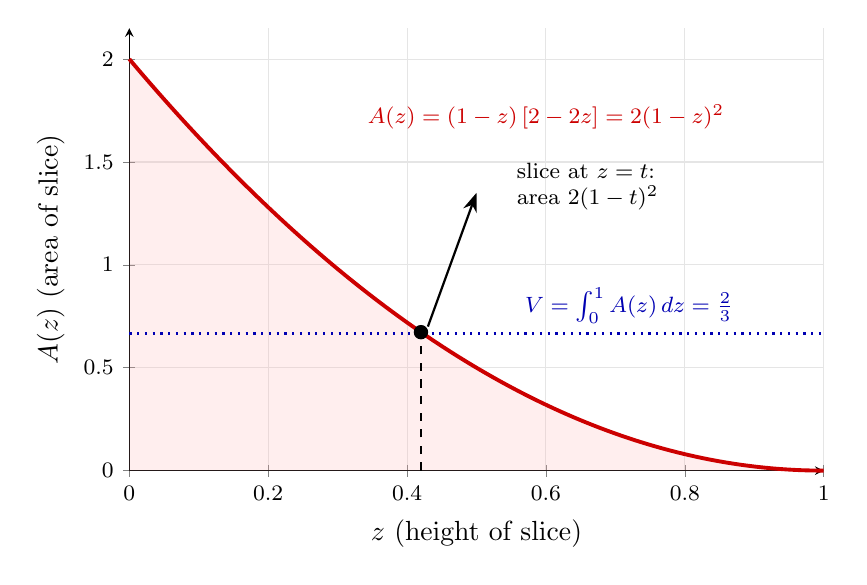
\begin{tikzpicture}
\begin{axis}[
    width=10.4cm, height=7.2cm,
    domain=0:1, samples=120,
    xmin=0, xmax=1, ymin=0, ymax=2.15,
    xtick={0,0.2,...,1.0}, ytick={0,0.5,...,2.0},
    tick label style={font=\footnotesize},
    xlabel={$z$ (height of slice)}, ylabel={$A(z)$ (area of slice)},
    grid=major, grid style={gray!20}, clip=false, axis lines=left,
    every node/.style={font=\small},
]
\addplot[fill=red!30, fill opacity=.22, draw=none] {2*(1-x)^2} \closedcycle;
\addplot[red!80!black, line width=1.4pt] {2*(1-x)^2};
\node[red!80!black, align=left, font=\footnotesize] at (axis cs:0.60,1.72)
     {$A(z)=(1-z)\,[2-2z]=2(1-z)^2$};

\draw[dashed, thick, black] (axis cs:0.42,0) -- (axis cs:0.42,0.6728);
\addplot[only marks, mark=*, mark size=2.4pt, black] coordinates {(0.42,0.6728)};
\draw[{Stealth[length=2.4mm]}-, thick, black] (axis cs:0.50,1.35) -- (axis cs:0.43,0.70);
\node[align=left, font=\footnotesize] at (axis cs:0.66,1.38) {slice at $z=t$:\\ area $2(1-t)^2$};

\draw[dotted, thick, blue!70!black] (axis cs:0,0.6667) -- (axis cs:1,0.6667);
\node[blue!70!black, font=\footnotesize, above] at (axis cs:0.72,0.6667) {$V=\int_0^1 A(z)\,dz=\frac{2}{3}$};
\end{axis}
\end{tikzpicture}
\end{document}